\chapter{Brute Force Approach}

In the previous chapter the correlation between the solar-zenith angle's cosine and the estimated VTEC value was seen. In ths section we aim to provide a first, brute force approach, for an algorithm able to estimate the Sun's location based on this study. This first approach is done as a first approximation to be problem to see more clearly how the algorithm will work, regarless of the performance.

\section{Key elements}

\subsection{Correlation}

explain, formulas, references, etc

explain R and compare to show the computation is correct

\subsection{Moment of the flare}

The first part of the algorithm was, without going into the actual computations regarding the position of the IPPs, the possible Sun locations, etc, finding out when to perform the study, that is, detecting a spike in the VTEC content in general, for any IPP. In the previous chapter we knew the specific moment of the flare (11.05h), but the algorithm has to determine which moment is going to be studied.

A first approach to detecting thiswe first wanted to detect a spike in the VTEC content throughout the day in a simple way. For each epoch \footnote{In our data set the epochs ranged from 10.5 to 11.5, that it is, 10:30AM to 11:30AM with a sampling rate of 1/120 hours or 30 seconds} we computed the mean VTEC of all IPPs and inserted it into a priority queue. We did this because we wanted to see thbut a simple single-pass max-value finder would work

explicar buscar pico por hill climbing o algo asi usando la grafica de la distribucion. Al encontrar un momento exacto en el que centrarnos empezar a estudiar ahi

\subsection{Linking C++ and Fortran}

explicar aqui que la logica se hace con c++ y la computacion numerica con Fortran

\begin{lstlisting}[language=Python, caption=Python example]
import numpy as np

def incmatrix(genl1,genl2):
m = len(genl1)
n = len(genl2)
M = None #to become the incidence matrix
VT = np.zeros((n*m,1), int)  #dummy variable

#compute the bitwise xor matrix
M1 = bitxormatrix(genl1)
M2 = np.triu(bitxormatrix(genl2),1) 

for i in range(m-1):
for j in range(i+1, m):
[r,c] = np.where(M2 == M1[i,j])
for k in range(len(r)):
VT[(i)*n + r[k]] = 1;
VT[(i)*n + c[k]] = 1;
VT[(j)*n + r[k]] = 1;
VT[(j)*n + c[k]] = 1;

if M is None:
M = np.copy(VT)
else:
M = np.concatenate((M, VT), 1)

VT = np.zeros((n*m,1), int)

return M
\end{lstlisting}




\section{Brute force approach}

explicar que es para entender que debemos hacer

\subsection{Pseudocode}

primero pseudocodigo, explicar for each dec for each ra


\begin{algorithm}
	\caption{My algorithm}\label{euclid}
	\begin{algorithmic}[1]
		\Procedure{bruteForceAlgorithm}{}
		\State $\textit{stringlen} \gets \text{length of }\textit{string}$
		\State $i \gets \textit{patlen}$
		\BState \emph{top}:
		\If {$i > \textit{stringlen}$} \Return false
		\EndIf
		\State $j \gets \textit{patlen}$
		\BState \emph{loop}:
		\If {$\textit{string}(i) = \textit{path}(j)$}
		\State $j \gets j-1$.
		\State $i \gets i-1$.
		\State \textbf{goto} \emph{loop}.
		\State \textbf{close};
		\EndIf
		\State $i \gets i+\max(\textit{delta}_1(\textit{string}(i)),\textit{delta}_2(j))$.
		\State \textbf{goto} \emph{top}.
		\EndProcedure
	\end{algorithmic}
\end{algorithm}

entonces explicar aqui lo de los polos, in a first approach to this in which to visually see ourselves the differences between possible Sun positions we obtained a plot for each possibility (figure \ref{fig:poles}), we could see this happening:

\begin{figure}[!htb]
	\begin{subfigure}[b]{0.5\textwidth}
		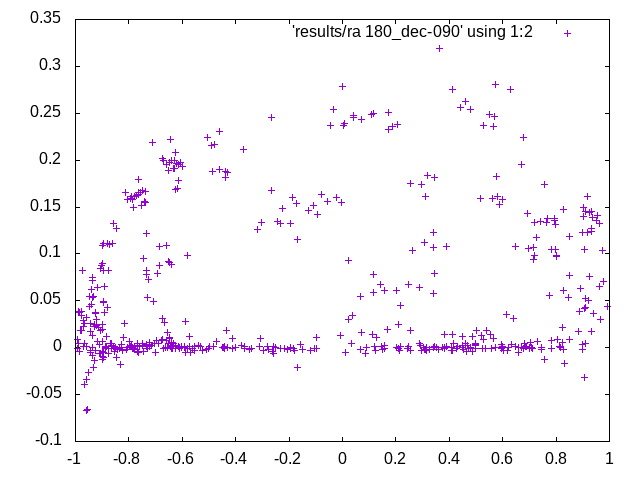
\includegraphics[width=\linewidth]{images/ch4/ra180_dec-090.png}
		\caption{ra180 and dec-090}
	\end{subfigure}
	\hfill
	\begin{subfigure}[b]{0.5\textwidth}
		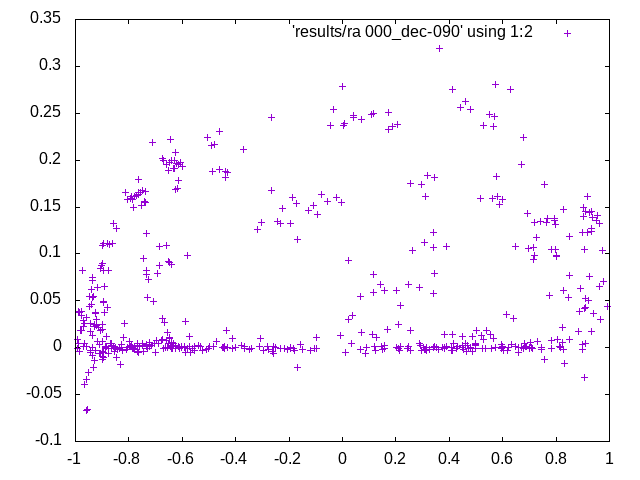
\includegraphics[width=\linewidth]{images/ch4/ra000_dec-090.png}
		\caption{ra000 and dec-090}
	\end{subfigure}
	\caption{dasdasdasda}
	\label{fig:poles}
\end{figure}

The two images are equivalent using the diff




\subsection{Results}

Comparison of precision and time here



\begin{lstlisting}[caption=Brute force approach algorithm output]
[C++: Finding a spike in the VTEC distribution]
[AWK: Filtering all data by best epoch: 11.05]
[C++ -> Fortran: Finding the Person coefficients for possible Suns | Epoch = 11.050000]
[C++ -> R: Computing correlation coefficient for each possible Sun with R]
[R: RESULTS] 
Largest correlation coefficient: 0.9073422 
Estimated Sun's location:  ra210_dec-010
\end{lstlisting}

As we can see this approach provides the expected results, but has a large computational complexity that increases with the precision we want to obtain in our results. In the next chapter, an algorithm is presented to perform this computations with several optimizations to reduce its complexity.